%%%%%%%%%%%%%%%%%%%%%%% file template.tex %%%%%%%%%%%%%%%%%%%%%%%%%
%
% This is a general template file for the LaTeX package SVJour3
% for Springer journals.          Springer Heidelberg 2010/09/16
%
% Copy it to a new file with a new name and use it as the basis
% for your article. Delete % signs as needed.
%
% This template includes a few options for different layouts and
% content for various journals. Please consult a previous issue of
% your journal as needed.
%
%%%%%%%%%%%%%%%%%%%%%%%%%%%%%%%%%%%%%%%%%%%%%%%%%%%%%%%%%%%%%%%%%%%
%
% First comes an example EPS file -- just ignore it and
% proceed on the \documentclass line
% your LaTeX will extract the file if required
\begin{filecontents*}{example.eps}
%!PS-Adobe-3.0 EPSF-3.0
%%BoundingBox: 19 19 221 221
%%CreationDate: Mon Sep 29 1997
%%Creator: programmed by hand (JK)
%%EndComments
gsave
newpath
  20 20 moveto
  20 220 lineto
  220 220 lineto
  220 20 lineto
closepath
2 setlinewidth
gsave
  .4 setgray fill
grestore
stroke
grestore
\end{filecontents*}
%
\RequirePackage{fix-cm}
%
\documentclass{svjour3}                     % onecolumn (standard format)
%\documentclass[smallcondensed]{svjour3}     % onecolumn (ditto)
%\documentclass[smallextended]{svjour3}       % onecolumn (second format)
%\documentclass[twocolumn]{svjour3}          % twocolumn
%
\smartqed  % flush right qed marks, e.g. at end of proof
%
\usepackage{graphicx}
%
% \usepackage{mathptmx}      % use Times fonts if available on your TeX system
%
% insert here the call for the packages your document requires
%\usepackage{latexsym}
% etc.
%
% please place your own definitions here and don't use \def but
% \newcommand{}{}
%
% Insert the name of "your journal" with
% \journalname{myjournal}
%
\begin{document}

\title{Lab Report - Reinforcement Learning Project %\thanks{Grants or other
%notes about the article that should go on the front page should be
%placed here. General acknowledgments should be placed at the end of the article.}
}
%\subtitle{Do you have a subtitle?\\ If so, write it here}

%\titlerunning{Short form of title}        % if too long for running head

\author{Janosch Moos         \and
        Kay Hansel           \and
        Cedric Derstroff
}

%\authorrunning{Short form of author list} % if too long for running head

\institute{C. Derstroff \at
          \email{cedric.derstroff@stud.tu-darmstadt.de}           %  \\
%             \emph{Present address:} of F. Author  %  if needed
           \and
           J. Moos \at
           \email{janosch.moos@stud.tu-darmstadt.de}
           \and
           K. Hansel \at
           \email{kay.hansel@stud.tu-darmstadt.de}
}

\date{Received: date / Accepted: date}
% The correct dates will be entered by the editor


\maketitle

\begin{abstract}
Insert your abstract here. Include keywords, PACS and mathematical
subject classification numbers as needed.
\keywords{Furuta Pendulum \and Cartpole \and Inverted Pendulum \and Ball Balancer \and Classical Control \and Artificial Intelligence \and Reinforcement Learning \and NPG \and NES}
% \PACS{PACS code1 \and PACS code2 \and more}
% \subclass{MSC code1 \and MSC code2 \and more}
\end{abstract}

\section{Introduction}
\label{intro}
The field of Reinforcement Learning is progressing further and further. A lot of algorithms have been published over the past years using various approaches to solve black box problems \cite{Wierstra14}. For this project, we have been assigned the task to implement the Natural Policy Gradient (NPG) \cite{Rajeswaran2017,Kakade2001} and the Natural Evolution Strategies (NES) \cite{Wierstra14}. To evaluate their performance we also have been assigned two platforms, the Cartpole and the Furuta Pendulum. Three tasks have to be solved on these platforms including the Cartpole swing up, the Cartpole double pendulum stabilization and the Furuta pendulum swing up \cite{Furuta1991}. We will discuss these platforms and tasks further in \autoref{plats} to show how they work. In this report we will shortly introduce the algorithms, platforms. Afterward, we will present our results and findings.

\subsection{Algorithms}
\label{algos}
Reinforcement Learning can be defined by various different optimization problems. One of them is to use a trajectory-based approach
\begin{align}
  J(\pi) = \int_{\mathbb{T}} p^{\pi}(\tau) r(\tau) d\tau.
\end{align}
By formulating the derivatives and applying the logarithm likelihood trick we can derive the "vanilla gradient" or REINFORCE algorithm \cite{Williams1992}
\begin{align}
  \nabla_{\theta} J(\pi) = \int_{\mathbb{T}} p^{\pi}(\tau) \nabla_{\theta} \log p^{\pi}(\tau) r(\tau) d\tau \approx \frac{1}{N} \sum_{i=1}^{N} \nabla_{\theta} \log p^{\pi}(\tau_i) r(\tau_i).
\end{align}
If we now add a constraint to regularize the gradients we can rewrite the optimization problem as
\begin{align}
  \max_{\delta\theta} \hat J(\theta + \Delta\theta) &= J(\theta) + \nabla_{\theta} J^T \Delta\theta \nonumber \\
  s.t. \ D(p_{\theta + \Delta\theta} || p_{\theta}) &= \Delta\theta^T F(\theta) \Delta\theta \leq \epsilon \label{NpgOpti}
\end{align}
with the Fisher information matrix $F$. This leads to the natural gradient $F^{-1} \nabla_{\theta} J$ \cite{Rajeswaran2017}
\begin{align}
  \Delta \theta = \alpha F^{-1} \nabla_{\theta} J = \sqrt{\frac{\delta}{\nabla_{\theta} J^T F^{-1} \nabla_{\theta} J}} F^{-1} \nabla_{\theta} J.
\end{align}
As a first setup, we implemented the NPG as described in \cite{Rajeswaran2017} which however led to a lot of problems while calculating the Fisher information matrix (FIM). Not only is calculating the FIM computationally expensive, but it can also result in uninvertible matrices \cite{DuanCHSA16}. To get around these problems we decided to use conjugate gradients to compute the natural gradient \cite{DuanCHSA16}. To further increase the efficiency we also added importance sampling, which brought us from NPG to the Trust Region Policy Optimization (TRPO) \cite{SchulmanLMJA15,Telesens}. In this context, we switched to neural network based gaussian policy. To prevent confusion we will still denote to this as NPG in this report.\\

In contrast of the NPG, the algorithms of the NES family utilize a search distribution over the parameters $\theta$. Each episode a batch of sample parameters $z$ is drawn from this distribution. These samples are used to run a trajectory which is evaluated with a fitness function $f(z)$. We can formalize this as an optimization function
\begin{align}
  J(\theta) = \int f(z) \pi(z|\theta) dz
\end{align}
which leads to an estimate of the search gradients from samples $z_1 ... z_{\lambda}$
\begin{align}
  \nabla_{\theta} J \approx \frac{1}{\lambda} \sum_{k=1}^{\lambda} f(z_k) \nabla_{\theta} \log \pi(z_k|\theta)
\end{align}
with population size $\lambda$ \cite{Wierstra14}. \\
The first version we implemented was the Canonical NES \cite{Wierstra14}. Similar to the NPG it adds a constraint to the optimization to regularize the gradients as in  \autoref{NpgOpti}. However as already described above we ran into problems while calculating the FIM. To avoid the same struggles as in the NPG we decided to switch to another version of the NES called Separable NES (SNES), which changes the update complexity from quadratic to linear \cite{Wierstra14}.

\subsection{Platforms}
\label{plats}
The algorithms have to be tested and evaluated on at least three different tasks. Two of these, the Cartpole swing up and the double pendulum stabilization, are executed on the Cartpole platform. The third task runs on the Furuta Pendulum \cite{Furuta1991}. \\

The Cartpole is a fairly simple mechanical system. It consists of a sled which can move left and right on a rail. Connected to the sled is a stiff rod swinging freely whenever the sled moves \cite{Barto1983}. There are several variations of tasks that can be performed on the Cartpole platform ranging from simple stabilization of a single rod to more complex tasks like stabilizing two, three or even four rods stacked on top of each other connected by free links. An even more challenging task is the swing up. Starting in a hanging position the rod has to be swung up and stabilized afterward. The complexity can be increased further by stacking more rods similar to before. \\

The Furuta Pendulum is a rotary inverted pendulum invented by Katsuhisa Furuta and his colleagues in 1991 \cite{Furuta1991}. It is an underactuated, non-linear system with a stiff rod attached to a single motor by a rigid link. The motor rotates the rod in a horizontal plane. Attached to the other end of the rod is a free link with a second rod perpendicular to the first. When the motor moves the first rod, the second one rotates in a vertical plane always perpendicular to the first rod. Compared to the Cartpole system it provides multiple advantages such as using less experimental space and having fewer uncertainties in the mechanical transmission system \cite{Furuta1991}. The task here is to use the rotation of the motor to swing up the second rod and stabilize it. Similar to the Cartpole the complexity can be increased by stacking more rods with free links onto the second one in the same direction.

\section{Results}
\label{results}
During our experiments, we observed that there is a huge difference in the policy behavior between the simulation and physical system. Often there will be policies running flawlessly in simulation but are unable to solve the problem even closely in reality. Further, NPG and NES behave quite differently during their training. Thus, in order to present and discuss our findings, we will split this section into two parts, Simulation and Physical System.

\subsection{Simulation}
\label{sim}

\begin{figure*}
\centering
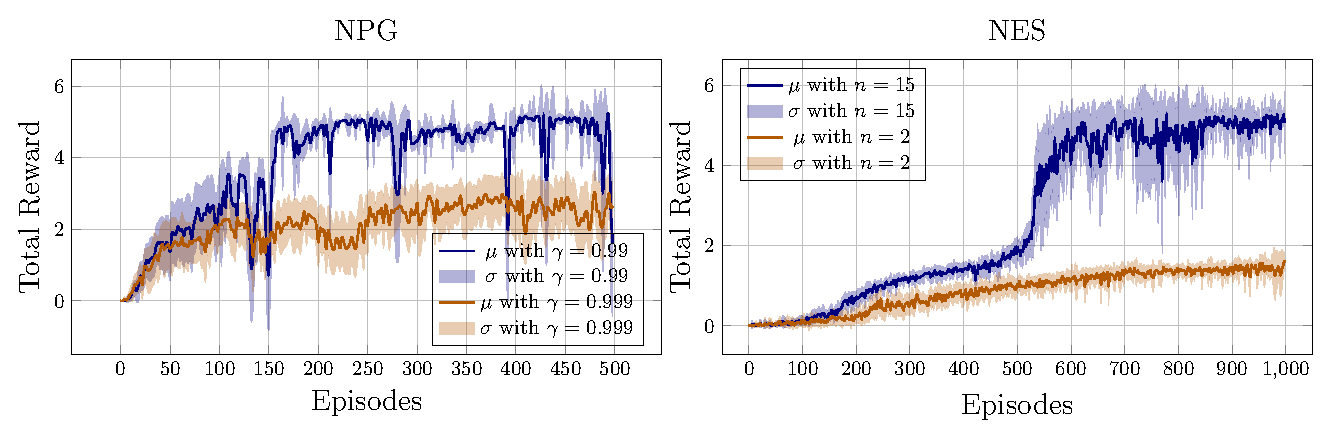
\includegraphics[scale=.5]{plots/qube_compare.pdf}
\caption{Comparison of the training process with different hyperparameters. The plots show the huge impact even a single hyperparameter can have on the training process.}
\label{fig:NPG_training}
\end{figure*}

Training a policy with the NPG turned out to be quite difficult. The biggest hurdle is finding suitable hyperparameters. \autoref{fig:NPG_training} shows the training process of the NPG on the left and NES on the right with two different sets of hyperparameters each. For the NPG we chose to change the discount factor $\gamma$, however, this is only one of many hyperparameters that can be changed in order to solve the optimization problem. \newpage
The most important parameters are:
\begin{itemize}
  \item Trust Region $\delta$: \\
  $\delta$ regulates the step size of the policy update which can lead to faster convergence. However, this can also result in worse performance because the algorithm may not converge to a global optimum and instead jumps among suboptimal solutions. We also observed that for varying $\delta$ we can get large jumps in performance during the training process as evident in the top left of \autoref{fig:NPG_final} \smallskip
  \item Discount Factor $\gamma$: \\
  $\gamma$ determines the focus to short or long term rewards. Increasing the value also increases the importance of long term reward and vice versa \cite{Schulman2018}. \smallskip
  \item $\lambda$: \\
  $\lambda$ is used to realize a tradeoff between bias and variance in the advantage estimation \cite{Schulman2018}. \smallskip
  \item Number of rollouts $n$: \\
  A higher number of rollouts per episode decreases the variance between episodes as the distribution over possible starting positions is averaged more realistically.\smallskip
  \item Policy $\pi$: \\
  The policy maps states to actions. As such depending on the tasks to solve different policy classes can be applied \cite{Rajeswaran2017}. For our implementation, we only use a neural network based gaussian policy, which not only the NPG, as implemented at this point, is efficient for, but also makes feature construction unnecessary. For our project, we decided to use the Adam optimizer as well as the $\tanh$ activation function, however, the activation function can also be changed if needed. The main difficulty is to find the right network size. \smallskip
  \item Baseline $b$: \\
  The baseline estimates the state-value function. Possibly every regression algorithm can be used to realize the estimation provided suitable features are used. To simplify the implementation, we decided to represent the baseline with a neural network as well. In order to increase its performance, we added batch normalization. As such the baseline itself has multiple parameters that can be changed. The network size and number of epochs are our main concern. The batch size is set to 64 as default but can be adjusted as well as the learning rate which is set to $10^{-3}$. The optimizer and activation is the same as in the policy network. Despite fixing the optimizer, we noticed during our experiments that the optimizer has a huge impact. Adam behaves very differently to e.g. the SGD.
\end{itemize}
\begin{figure*}
\centering
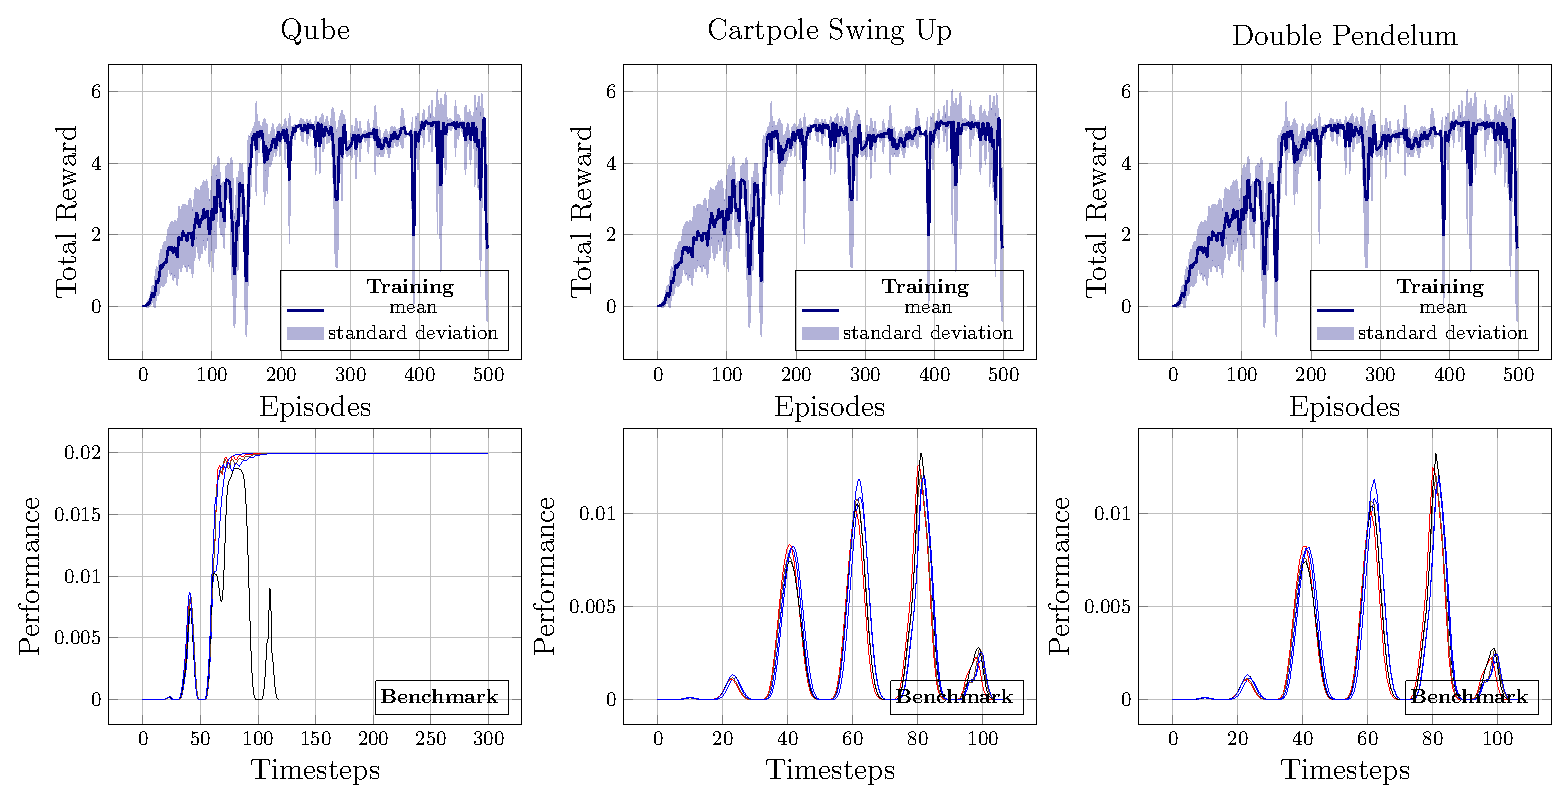
\includegraphics[width=\textwidth]{plots/learned_benchmarked_NPG.pdf}
\caption{This figure shows the training process of the NPG as well as a benchmark with the final policy on each of the three tasks described in \autoref{intro}. "Qube" is referring to the Furuta Pendulum.}
\label{fig:NPG_final}
\end{figure*}

\autoref{fig:NPG_final} shows our final results on the given tasks using the NPG. We recognized that the most important parameters are $\gamma$ and $\lambda$ of the advantage function. We have had a lot of trouble finding suitable parameters for the given tasks and, unfortunately, have not managed to solve the Cartpole swing up. \\
Another important insight is provided by the benchmark plots, which are shown in the lower row of \autoref{fig:NPG_final}. Each plot illustrates ten of the 100 runs of the benchmark test. It is important, depending on the environment, to perform a representative amount of runs, because the starting position can vary, which might lead to false positive results as pictured in the bottom left plot in \autoref{fig:NPG_final}. During one of the runs the simulation was terminated early because the robot hit the restriction in the movement space and did not manage to perform the swing up. To ensure the best performance the exploration was set to zero for the benchmarks. \\
In the produced experiments we have even encountered policies whose exploration converged to almost zero and thus the total reward of the last training episodes was close to the benchmark performance. This is the desired behavior of gaussian policies, which should converge to an optimal policy without further exploration after sufficient training with suitable hyperparameters (see \autoref{fig:NES_final} Double Pendulum). \\

\begin{figure*}
\centering
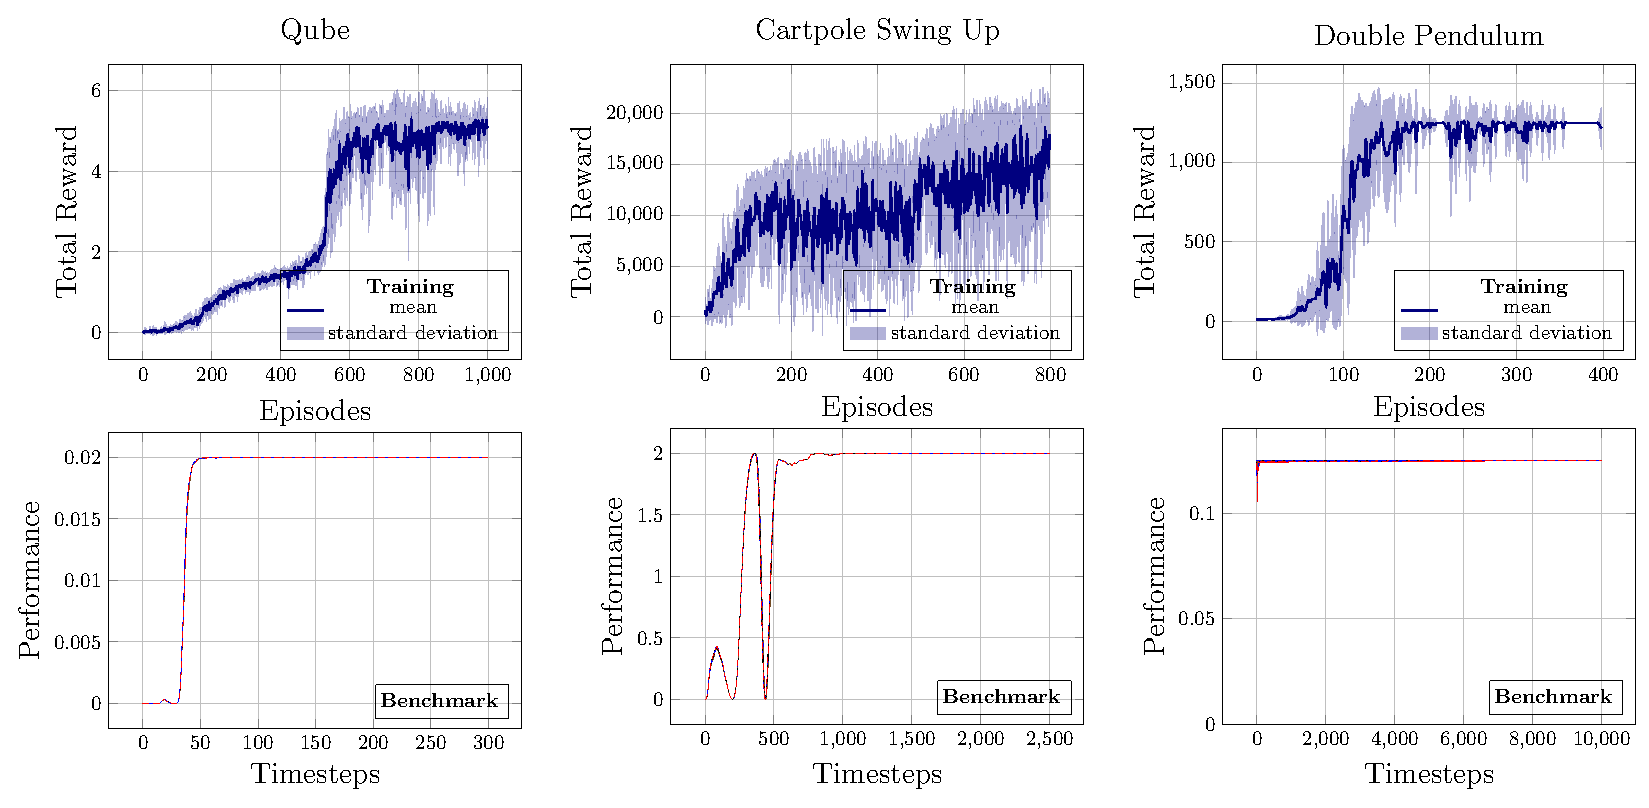
\includegraphics[width=\textwidth]{plots/learned_benchmarked_NES.pdf}
\caption{Final results for given tasks using SNES}
\label{fig:NES_final}
\end{figure*}

As already mentioned in \autoref{intro} with the Canonical NES we had similar problems as with the first version of the NPG. Inverting the FIM often resulted in singular matrices, but in addition, both were very slow. In the case of the NES, we decided to switch to the SNES, which turned out to be a huge success. \autoref{fig:NES_final} illustrates our final results with the SNES on all tasks. We managed to solve all platforms due to the fact that the SNES compared to the NPG has fewer hyperparameters that need to be adjusted. The only ones being:
\begin{itemize}
  \item Population size $\lambda$: \\
  The population size $\lambda$ defines the number of samples which are drawn from the search distribution for each episode. For all our solutions we used the calculation for $\lambda$ suggested by \cite{Wierstra14}. \smallskip
  \item Number of rollouts $n$: \\
  In the case of the NES, this parameter does not define the number of rollouts per episode but rather the rollouts performed for each policy evaluation. Thus, for each episode $\lambda \cdot n$ simulations are executed while resetting the environment seed between each sample to a random value chosen at the beginning of each episode. Increasing the number of rollouts decreases the variance during rollouts similar to the NPG. Our experiments have shown that for most platforms and tasks $n=2$ turned out to be enough to find good solutions. To solve the Furuta Pendulum, however, we had to use $n=15$ as it was much more unstable than the Cartpole These settings have also been used to produce the plots in \autoref{fig:NES_final}. \smallskip
  \item Policy $\pi$: \\
  Similar to the NPG the policy can be chosen arbitrarily depending on tasks and setup. We decided to use the greedy version of the policy we used for the NPG as the NES already incorporates exploration in the search distribution over the policy parameters. Additionally, we avoid the same problems using a neural network as described for the NPG. As such we have the same adjustable parameters for the NN, which however turned out not to be as impactful as in the NPG. For all tasks, we used a neural network with a single layer and 10 nodes and the default $\tanh$ activation function. \smallskip
  \item Fitness function $f(z)$: \\
  The fitness function is crucial to evaluate the performance of the sample policies $\pi_z$. There a many possible options to choose from. We decided to go with one of the easiest by using $f(z) = \sum_{k=1}^{n} \sum_{i=1}^{T} r_{k,t}$.
\end{itemize}

In the end the SNES was not only easier to implement but also much easier to handle and set up. It has a lot less crucial hyperparameters that need to be adjusted and in addition, it is also much more invariant to small changes in the hyperparameters. We have observed that even though the SNES takes much longer than the NPG to reduce its exploration to near zero it manages to converge much faster to a policy of high quality.

\subsection{Physical System}
\label{phys}
\vspace{-.8cm}
\begin{figure}[ht]
\centering
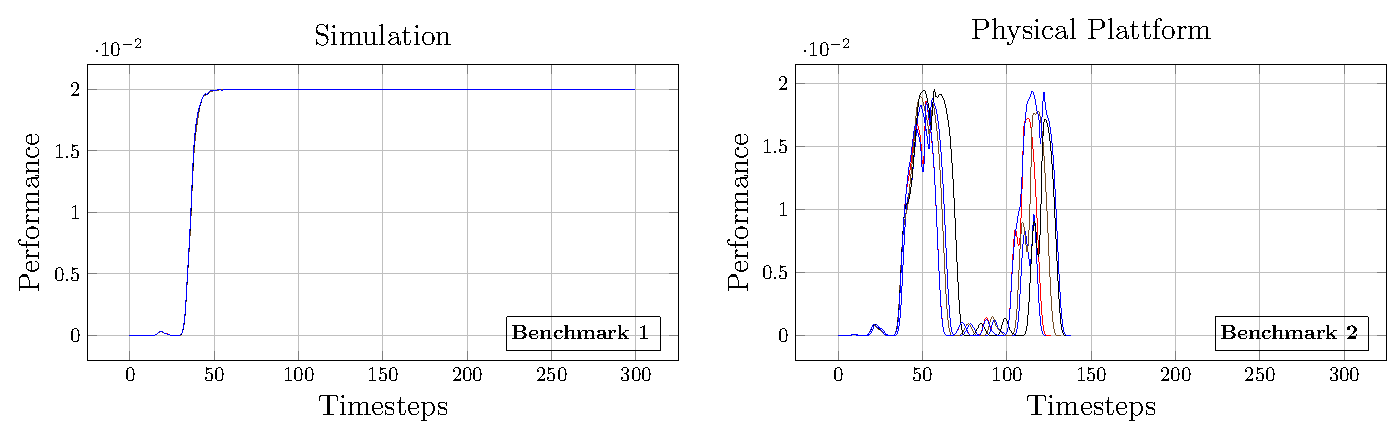
\includegraphics[scale=.5]{plots/nes_on_rr_master.pdf}
\caption{Trained policy using NES in simulation and applied to physical Qube}
\label{fig:NES_sim_to_physqube}
\end{figure}

Learning a policy in simulations is only the first step. In the end, we need to control a real physical system. Anyhow, applying a policy trained in simulation to a physical system can lead to tremendous drops in performance. \autoref{fig:NES_sim_to_physqube} pictures this drop in performance really well. As can be seen, the benchmark ran flawlessly in the simulation while crashing spectacularly on the physical system. We got a similar result for the NPG on the Furuta Pendulum. One reason we noticed was that the state space was slightly smaller in reality due to an obstacle mounted on the Qube to prevent damage when using suboptimal controllers. In order to apply policies without having this issue, we decided to clip the state space of the simulation to $[-\pi, \pi]$ and retrained the policies with both algorithms.

\begin{figure}[ht]
\centering
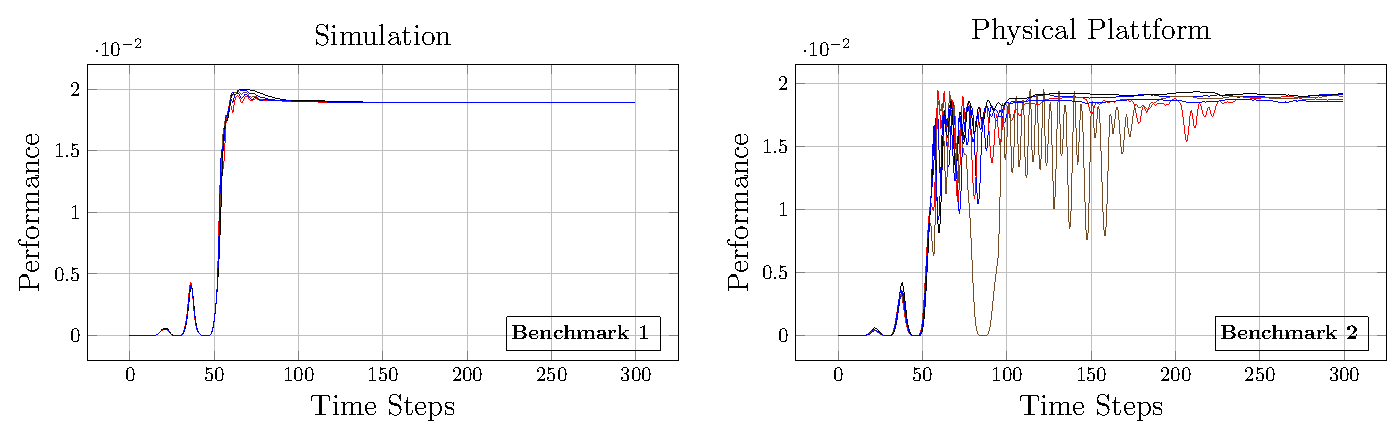
\includegraphics[scale=.5]{plots/npg_on_rr_master.pdf}
\caption{Policy performance using NPG and clipped state space}
\label{fig:NPG_sim_to_physqube}
\end{figure}

Applying the new policy learned with the NPG worked surprisingly well. \autoref{fig:NPG_sim_to_physqube} displays the benchmark results for our policy trained in the new state space. It is evident that the drops in performance were less sever than before. The NPG even managed to perform the swing up and stabilization of the Furuta Pendulum in all benchmark runs. However, when applying the NES we recognized that this is not the case for all policies as the NES policy did not perform a single swing up. Instead, with this particular NPG policy, we got lucky as it was not as efficient during the swing up period as the others. In \autoref{fig:NES_sim_to_physqube} and \ref{fig:NPG_sim_to_physqube} we notice the difference in the swing up of the simulation. The new NPG policy took longer to perform the swing up and used two instead of one swing before getting into an upright position while the new NES policy performed similarly to before as in \autoref{fig:NES_sim_to_physqube}. On that basis we conclude that most policies are trained to a point were they perform unrealistically good and thus are overfitted to the simulation.
So in order to train a good controller for real systems we can either train a policy in simulation and tune it on the physical system or train on the physical system from the start. Due to limited time we only used the first method.
Though while tuning the new NES policy on the real system we encountered a huge problem. Every few runs the system crashed without stopping the training process. Instead, when crashed, each run ended after few steps with almost no reward which made it nearly impossible to improve the policy. Due to this fact, we decided to try solving the real Cartpole swing up with the NES. Similar to the Qube the NES performed nearly perfectly in simulation and its performance dropped on the real Cartpole. \autoref{fig:NES_sim_to_physcart} shows the proccess of applying the NES to the Carpole in the first row while the second illustrates the improvement of the policy after 30 and 60 episodes. To prevent damage to the system we have clipped the actions to $[-6, 6]$. We also managed to solve the Ball-Balancer-v0 and Levitation-v0 with the same parameters using the NES, but did not include the results due to a lack of space.
\begin{figure}
\centering
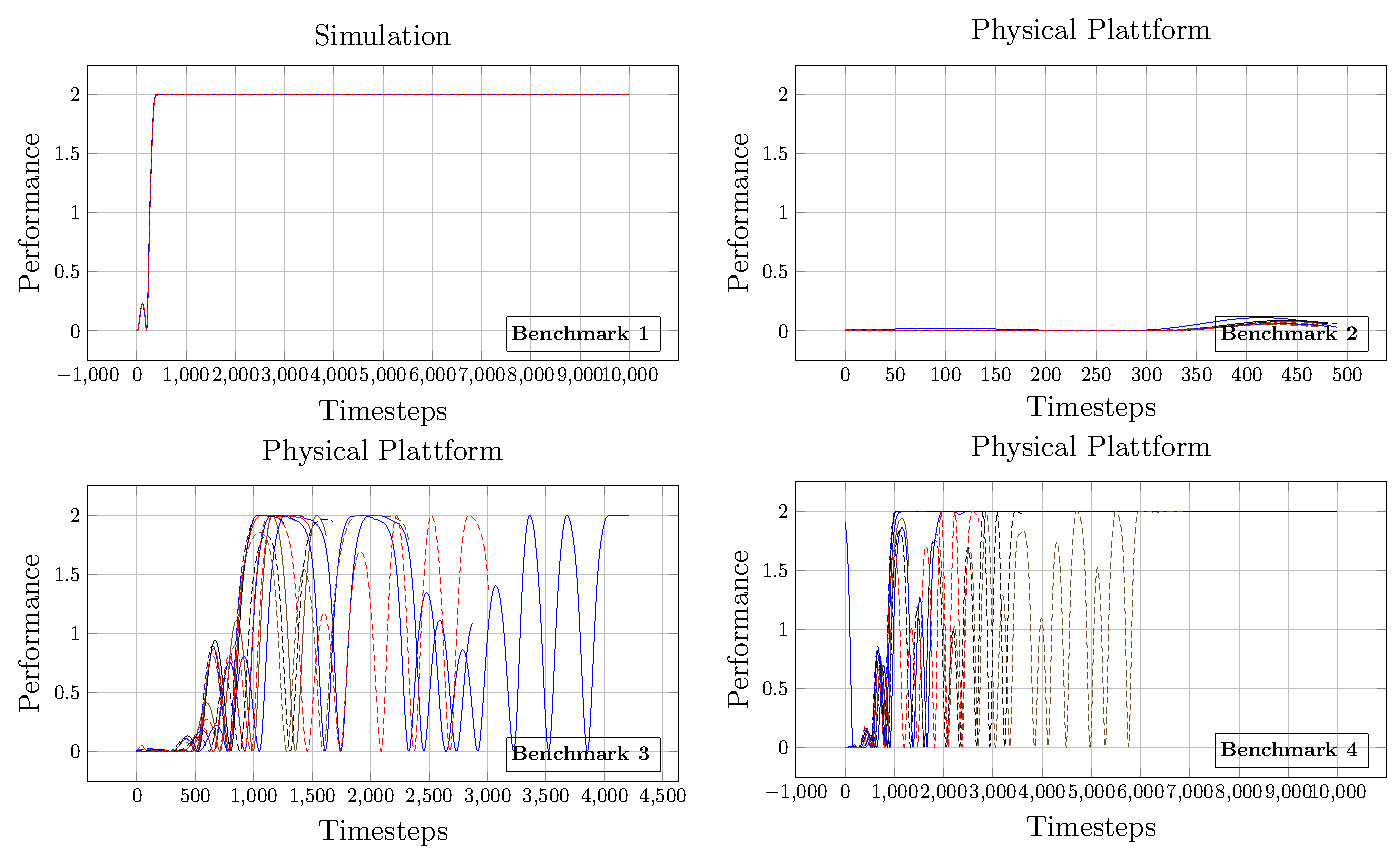
\includegraphics[scale=.5]{plots/training_on_rr.pdf}
\caption{Tuning of new NES policy on real Cartpole}
\label{fig:NES_sim_to_physcart}
\end{figure}


% \paragraph{Paragraph headings} Use paragraph headings as needed.
% \begin{equation}
% a^2+b^2=c^2
% \end{equation}

% % For one-column wide figures use
% \begin{figure}
% % Use the relevant command to insert your figure file.
% % For example, with the graphicx package use
%   
\includegraphics{example.eps}
% % figure caption is below the figure
% \caption{Please write your figure caption here}
% \label{fig:1}       % Give a unique label
% \end{figure}
% %
% % For two-column wide figures use
% \begin{figure*}
% % Use the relevant command to insert your figure file.
% % For example, with the graphicx package use
%   
\includegraphics[width=0.75\textwidth]{example.eps}
% % figure caption is below the figure
% \caption{Please write your figure caption here}
% \label{fig:2}       % Give a unique label
% \end{figure*}
% %
% % For tables use
% \begin{table}
% % table caption is above the table
% \caption{Please write your table caption here}
% \label{tab:1}       % Give a unique label
% % For LaTeX tables use
% \begin{tabular}{lll}
% \hline\noalign{\smallskip}
% first & second & third  \\
% \noalign{\smallskip}\hline\noalign{\smallskip}
% number & number & number \\
% number & number & number \\
% \noalign{\smallskip}\hline
% \end{tabular}
% \end{table}


%\begin{acknowledgements}
%If you'd like to thank anyone, place your comments here
%and remove the percent signs.
%\end{acknowledgements}

% BibTeX users please use one of
%\bibliographystyle{spbasic}      % basic style, author-year citations
%\bibliographystyle{spmpsci}      % mathematics and physical sciences
%\bibliographystyle{spphys}       % APS-like style for physics
%\bibliography{}   % name your BibTeX data base

% Non-BibTeX users please use
\begin{thebibliography}{}
%
% and use \bibitem to create references. Consult the Instructions
% for authors for reference list style.
%
\bibitem{Furuta91}
Katsuhisa Furuta, Masaki Yamakita, Seiichi Kobayashi, Swing Up Control of Inverted Pendulum, IEEE, 1991
\bibitem{Furuta92}
Katsuhisa Furuta, Masaki Yamakita, Seiichi Kobayashi, Swing-Up Control of Inverted Pendulum using Pseudo-State Feedback, Journal of Systems and Control Engineering, 206, 263-269, 1992
\bibitem{MIT}
Andrew Careaga Houck, Robert Kevin Katzschmann, Joao Luiz Almeida Souza Ramos, Furuta Pendulum, MIT, 2013
\bibitem{Lund}
Magnus Gäfvert, Modelling the Furuta Pendulum, Lund Institute of Technology, 1998
\bibitem{PredictiveC}
Pavol Seman, Boris Rohal'-Ilkiv, Martin Juhás, Michal Salaj, Swinging up the Furuta Pendulum and its stabilization via model predictive control, Journal of Electrical Engineering, Vol. 64, 152-158, 2013
\bibitem{OnTheDynamics}
Benjamin Seth Cazzolato and Zebb Prime, On the Dynamics of the Furuta Pendulum, Journal of Control Science and Engineering, Vol. 2011, , 2011
\bibitem{NES}
Wierstra et. al., Natural Evolution Strategies, Journal of Machine Learning Research, Vol. 15, 949-980, 2014


% \bibitem{RefJ}
% Format for Journal Reference
% Author, Article title, Journal, Volume, page numbers (year)
% Format for books
% \bibitem{RefB}
% Author, Book title, page numbers. Publisher, place (year)
% etc
\end{thebibliography}

\end{document}
% end of file template.tex
